
% The \phantomsection command is needed to create a link to a place in the document that is not a
% figure, equation, table, section, subsection, chapter, etc.
% https://tex.stackexchange.com/questions/44088/when-do-i-need-to-invoke-phantomsection
\phantomsection

\chapter{Experiments}\label{chap:experiments}

To address the objective of this dissertation, experiments are conducted to evaluate learning-based primal heuristics for Mixed-Integer Linear Programming (MILP).
The ONTS problem (see Chap.~\ref{chap:onts}) serves as a realistic application to benchmark the selected techniques.

As discussed in Section~\ref{sec:onts-problem-statement}, during mission execution (with the nanosatellite in orbit), a new schedule must be generated during the communication window.
This involves optimizing multiple instances of the ONTS problem, given varying sets of tasks and updated nanosatellite information.
Each set of tasks is evaluated based on the resulting schedule, in an iterative process of including new tasks until scheduling becomes infeasible.
Therefore, during the communication window, quickly finding a good solution to a problem instance is more crucial than finding an optimal solution.
In other words, an efficient heuristic is crucial to allow for more iterations, which leads to a better set of tasks scheduled for execution.

The remaining of this chapter details the development and the experiments with the proposed learning-based heuristics for the ONTS problem.
This includes data acquisition, solution prediction model architecture, model training, and experiment setup.
Furthermore, the performance of the proposed learning-based heuristics is assessed on realistic instances of the ONTS problem.


\section{Data}

High-quality data is necessary both to train solution prediction models and to evaluate the proposed learning-based heuristics for the ONTS problem.
The datasets for both training and evaluation must be composed of instance-solution pairs, as discussed in Sec.~\ref{sec:training-solution-prediction}.
The quality of these instance-solution pairs is measured through their faithfulness, both the instance with respect to the true data distribution, and the solution with respect to the optimal.

\subsection{Instance space: the FloripaSat I mission}\label{sec:instance-space}

The instance space is defined from the parameters of the FloripaSat-I mission~\cite{marcelinoCriticalEmbeddedSystem2020}.
Their nanosatellite is in orbit at an altitude of 628 kilometers and an orbital period of 97.2 minutes.
The planning horizon is fixed at $T=125$ time slots, with one slot per minute, to account for a continuous scheduling, allowing for task executions that extend the communication window.
Any instance $I\in \mathcal{I}$ has either 9, 13, 18, 20, 22, or 24 tasks.

Once the orbit of the FloripaSat-I is stable and its received solar flux is constant, the power input vector $\bm{r}$ can be calculated deterministically from solar irradiance measurements as in \citeonline{morschfilhoComprehensiveAttitudeFormulation2020}.
Two years of solar irradiance data are used as a basis for the power input vectors of the instances in the instance space.
The set $R$ is used to denote all possible values of $\bm{r}$ from the historical data.
The other battery-related parameters (see Sec.~\ref{sec:onts-milp-formulation}) are fixed as 
\begin{align*}
    e &= 0.9 \\
    Q &= 5 \\
    \gamma &= 5 \\
    V_b &= 3.6 \\
    \rho &= 0.0
\end{align*}

The remaining parameters are constrained to ranges that match previous works in the area~\cite{rigoBranchandpriceAlgorithmNanosatellite2022,semanEnergyAwareTaskScheduling2022,rigoTaskSchedulingOptimal2021}.
Therefore, following the notation established in Sec.~\ref{sec:onts-milp-formulation}, the parameter space is defined as
\begin{equation}\label{eq:parameter-space}
\Pi = \bigcup_{\substack{J \in \left\{ 9,13,18,20,22,24 \right\} \\ T \in \left\{ 125 \right\} }} \Pi^{J,T}
,\end{equation}
where each $\Pi^{J,T}$ is a set of a parameter vectors \[
\pi_I= \left( \bm{u}, \bm{q}, \bm{y}^{\min}, \bm{y}^{\max}, \bm{t}^{\min}, \bm{t}^{\max}, \bm{p}^{\min}, \bm{p}^{\max}, \bm{w}^{\min}, \bm{w}^{\max}, \bm{r}, \rho, e, Q, \gamma, V_b \right) \in \Pi^{J,T}
\] such that
\begin{equation*}
\begin{aligned}
&\begin{rcases}
    & u_j \in [1, J] \\
	 & q_j \in [0.3, 2.5] \\
    	 & y_j^{\min} \in [1, \lceil T/45 \rceil] \\
    	 & y_j^{\max} \in [y_j^{\min}, \lceil T/15 \rceil] \\
    	 & t_j^{\min} \in [1, \lceil T/10 \rceil] \\
    	 & t_j^{\max} \in [t_j^{\min}, \lceil T/4 \rceil] \\
    	 & p_j^{\min} \in [t_j^{\min}, \lceil T/4 \rceil] \\
    	 & p_j^{\max} \in [p_j^{\min}, T] \\
    	 & w_j^{\min} \in [0, \lceil T/5 \rceil] \\
    	 & w_j^{\max} \in [\lfloor T-\lceil T/5 \rceil \rfloor, T]
\end{rcases} \forall j =1,\ldots,J \\
    &\quad \bm{r} \in R ,\, e = 0.9 ,\, Q = 5 ,\, \gamma = 5 ,\, V_b = 3.6 ,\, \rho = 0.0
.\end{aligned}
\end{equation*}
Finally, the input space is then defined from the parameter space, such that \[
    I\in \mathcal{I} \iff \pi_I \in \Pi 
.\] 


\subsection{Data acquisition}\label{sec:data-acquisition}

As historical data is not available for the ONTS problem, the dataset is built from randomly generated instances sampled uniformly from the instance space of the FloripaSat-I mission.
More precisely, the dataset is built with instances drawn uniformly from the instance space defined above.

As the addition of an element to the dataset requires a solution to the ONTS problem, the computational cost of building a large dataset with hard instances is very high.
To alleviate this cost, the training set is built solely with instances with fewer tasks, which are, on average, faster to solve than instances with many tasks.
However, the instances of interest are those with plenty of tasks, which are harder to solve in practice, and, thus, motivate the use of heuristics.
Therefore, the validation and test datasets are built from instances with many tasks, which are, on average, significantly harder to solve.
Table~\ref{tab:dataset} details the number of instances by size (number of tasks) in each dataset generated.

\begin{table}[h]
    \centering
    \caption{Number of instances by size in each dataset. The datasets were generated through Algorithm~\ref{alg:dataset-generation}.}
    \label{tab:dataset}
    \begin{tabular}{l | c | c | c}
    \toprule
    & Training & Validation & Test \\
    \midrule
    $J = 9$ & 200 & 0 & 0 \\
    $J = 13$ & 200 & 0 & 0 \\
    $J = 18$ & 200 & 0 & 0 \\
    $J = 20$ & 0 & 20 & 20 \\
    $J = 22$ & 0 & 20 & 20 \\
    $J = 24$ & 0 & 20 & 20 \\
    \midrule
    Total & 600 & 60 & 60 \\
    \bottomrule
    \end{tabular}
\end{table}

Distinguishing the size of the instances in each dataset allows for the construction of a large training set, which enables the models to properly learn the problem, while maintaining a challenging evaluation scenario.
On top of that, this approach also enables the evaluation of the generalization capabilities of the proposed solution prediction models and the derived learning-based heuristics.

The algorithm to generate the datasets is presented in Algorithm~\ref{alg:dataset-generation}.
Note that an instance is rejected if no feasible solution is found during the time budget or if the solver proves infeasibility.
As the time horizon is fixed, the algorithm is executed once for each number of tasks.
Similar to the parameter space definition \eqref{eq:parameter-space}, the resulting dataset can be described as
\begin{equation}\label{eq:dataset}
    \mathcal{D} = \bigcup_{\substack{J \in \left\{ 9,13,18,20,22,24 \right\} \\ T \in \left\{ 125 \right\} }}  \mathcal{D}^{(J,T)}
,\end{equation}
where each $\mathcal{D}^{(J,T)}$ is obtained through Algorithm~\ref{alg:dataset-generation}.
The algorithm is such that each element of the output dataset $(I,Z^\star_I) \in \mathcal{D}^{(J,T)}$ is composed of a \emph{feasible} instance $I$ sampled uniformly from the parameter space (see Eq.~\eqref{eq:parameter-space}) and deemed feasible by an MILP solver.
Furthermore, the accompanying set $Z^\star_I$ contains the best solutions found by the solver, which are necessary for training the model with multiple solutions as a target (see Sec. \ref{sec:multiple-targets}).

For our experiments, the algorithm was executed such that every new instance $I$ was solved using the SCIP solver~\cite{bestuzhevaSCIPOptimizationSuite2021} with a limited time budget of 5 minutes.
The best 500 solutions of each instance $I$ were recorded, i.e., for every $(I,Z^{*}) \in \mathcal{D}$, $|Z^{*}_I| = 500$.
Finally, the dataset is divided as $\mathcal{D} = \mathcal{D}_\textrm{train} \cup \mathcal{D}_{\textrm{val}} \cup \mathcal{D}_\textrm{test}$ following Table~\ref{tab:dataset}.

\begin{algorithm}[h]
    \NoCaptionOfAlgo
    \SetAlgoLined
    \KwData{Time horizon $T$, number of jobs $J$, number of instances (final dataset size) $n$.}
    \KwResult{Dataset $\mathcal{D}^{(J,T)} = \{(I,Z_I^\star): Z_I^\star\subset Z_I\}$.}
    
    \While{$|\mathcal{D}^{(J,T)}| < n$}{
        $\pi \sim \mathcal{U}\left( \Pi^{J,T} \right) $ \\
        $I \gets {\tt ONTS}(\pi)$ \\
        $Z_I^\star \gets {\tt Solver}(I)$
        
        \If{$|Z_I^\star| > 0$}{%
            $\mathcal{D}^{(J,T)}$.add$(I, Z_I^\star)$
        }
    }
    \caption{\textbf{Algorithm 1:} Dataset generation algorithm. $\pi$ is the parameter vector and $\Pi^{J,T}$ is the parameter space (see Sec. \ref{sec:onts-milp-formulation}), $Z_I$ represents the set of all feasible solutions of instance $I$, and $Z_I^\star \subset Z_I$ the set of feasible solutions the solver finds.
    ${\tt ONTS}$ represents a function that takes as input a parameter vector and constructs an instance of the ONTS problem.
    ${\tt Solver}$ is any MILP solver.
    Note that the parameters are drawn uniformly from the parameter space.
    }\label{alg:dataset-generation}
\end{algorithm}

\section{Solution Prediction Model}

The instance space of the ONTS problem, as defined in Sec.~\ref{sec:instance-space}, imposes specific architectural requirements for solution prediction models.
The variable number of tasks over the instances of interest leads to parameter vectors of variable length, which is a natural embedding (feature vector) for the instances.
At the same time, the uneven number of tasks in the instance space implies that instances have different number of binary variables.
Therefore, models must predict a different number of variable assignments for each instance.

Graph Neural Networks (GNNs) are particularly promising in this context and are considered state-of-the-art for such applications~\cite{cappartCombinatorialOptimizationReasoning2022}.
As discussed in Sec.~\ref{sec:gnns}, GNNs naturally handle variable input and output sizes due to their convolutional nature.
On top of that, results shown by \citeonline{gasseExactCombinatorialOptimization2019} point that GNNs are capable of generalizing to instances larger than those seen during training, which alleviates data acquisition costs, as discussed in Sec.~\ref{sec:data-acquisition}.
Therefore, the deep learning models trained for the ONTS problem are all built with GNNs at their core.

\subsection{Instance embedding}

Because GNNs are at the core of the solution prediction models, the instances are embedded as bipartite graphs, following the approach presented in~Sec.~\ref{sec:graph-embedding}.
Many authors have presented different approaches for defining node features when applying GNNs to MILP problems.
\citeonline{khalilMIPGNNDataDrivenFramework2022} add variable and constraint degrees\footnote{A variable's degree is the number of constraints in which it has a nonzero coefficient. On the other hand, a constraint's degree is the number of variables in it with non-zero coefficient.} to the baseline (the one presented in Sec.~\ref{sec:graph-embedding}) embedding.
\citeonline{chenRepresentingMixedIntegerLinear2022} embeds variables' upper and lower bounds as well as constraint type (inequality or equality).
Works that applied GNNs to generate branch-and-bound heuristics (e.g., for branching), such as \citeonline{dingAcceleratingPrimalSolution2020} and \citeonline{gasseExactCombinatorialOptimization2019}, have captured features usually available at the nodes of the branch-and-bound tree, directly collecting solver-computed features.
As the focus of the present work is on primal heuristics, the features should be solver-independent, i.e., they must be computed prior to the branch-and-bound application.

The resulting features used are based on the set proposed by \citeonline{hanGNNGuidedPredictandSearchFramework2023}, which extends both \citeonline{khalilMIPGNNDataDrivenFramework2022} and \citeonline{chenRepresentingMixedIntegerLinear2022} with simple features (solver-independent) that are also present in \citeonline{gasseExactCombinatorialOptimization2019}.
A summary is presented in Table~\ref{tab:feature-desc}.
Note that, following the literature, instead of describing all constraints as inequality constraints (i.e., in the normal form), the constraint type (inequality or equality) is informed through the constraint node features, reducing the graph size.
Furthermore, this feature design is problem agnostic, i.e., it does not use any information particular to the ONTS problem.

\begin{table}[h]
    \centering
    \begin{tabular}{p{7cm}|p{7cm}}
    \toprule
        Features of constraint nodes ($\bm{f}_{v_{\rm con}}$) & Features of variable nodes ($\bm{f}_{v_{\rm var}}$) \\
    \midrule
	Constraint's upper bound ($\bm{b}$)                     &  Variable's coefficient in the objective ($\bm{c}$)\\[0.8cm]
         Constraint's average coefficient (mean of $A_{i*}$)     &  Variable's average coefficient in the constraints (mean of $A_{*j}$) \\[0.8cm]
         Number of neighbors/non-null coefficients ($|\mathcal{N}(v_{\rm con})|$)    &  Number of neighbors/non-null coefficients ($|\mathcal{N}(v_{\rm var})|$) \\[0.8cm]
         Whether it is an equality or an inequality constraint &  Largest coefficient in the constraints ($\max(A_{*j})$) \\[0.8cm]
                                                                    &  Smallest coefficient in the constraints ($\min(A_{*j})$) \\[0.8cm]
                                                                    &  Whether it is a continuous or binary variable \\
    \bottomrule
    \end{tabular}
    \caption{Description of node features for the graph embedding of instances of the ONTS problem.}
    \label{tab:feature-desc}
\end{table}

\subsection{Architecture}

The structure of the solution prediction models is illustrated in Fig.~\ref{fig:satgnn}.
The model inputs are the embedding described in the previous section, i.e., the bipartite graph representation of the instance and the sets of feature vectors $F_\textrm{con}$ and $F_\textrm{var}$.
Each feature vector $\bm{f}_v$ is encoded into a hidden feature vector $\bm{h}^{(0)}_v$ with size $d$ by neural networks
\begin{align*}
    {\rm NN}_{\rm var}:\mathbb{R}^6& \longrightarrow\mathbb{R}^{d}_+ \\
    \bm{f}_{v_{\rm var}} &\longmapsto \bm{h}^{(0)}_{v_{\rm var}} = {\rm NN}_{\rm var}(\bm{f}_{v_{\rm var}})
\end{align*}
and
\begin{align*}
    {\rm NN}_{\rm con}:\mathbb{R}^4& \longrightarrow\mathbb{R}^{d}_+ \\
    \bm{f}_{v_{\rm con}} &\longmapsto \bm{h}^{(0)}_{v_{\rm con}} = {\rm NN}_{\rm con}(\bm{f}_{v_{\rm con}})
,\end{align*}
both with a single layer and ReLU (Rectified Linear Unit) activation~\cite{goodfellowQualitativelyCharacterizingNeural2015}.
More precisely, the first layer of hidden features of the GNN $H^{(0)}=\left\{ \bm{h}^{(0)}_v \in \R^{d} : v \in V \right\} $ is such that \[
\bm{h}^{(0)}_v = \begin{cases}
    {\rm NN}_{\rm con}(\bm{f}_v) & v \in V_\textrm{con} \\
    {\rm NN}_{\rm var}(\bm{f}_v) & v \in V_\textrm{var}
\end{cases}
.\] 
% Note that this operation makes all initial hidden features have the same dimension $d$.

\begin{figure}[h]
    \centering
    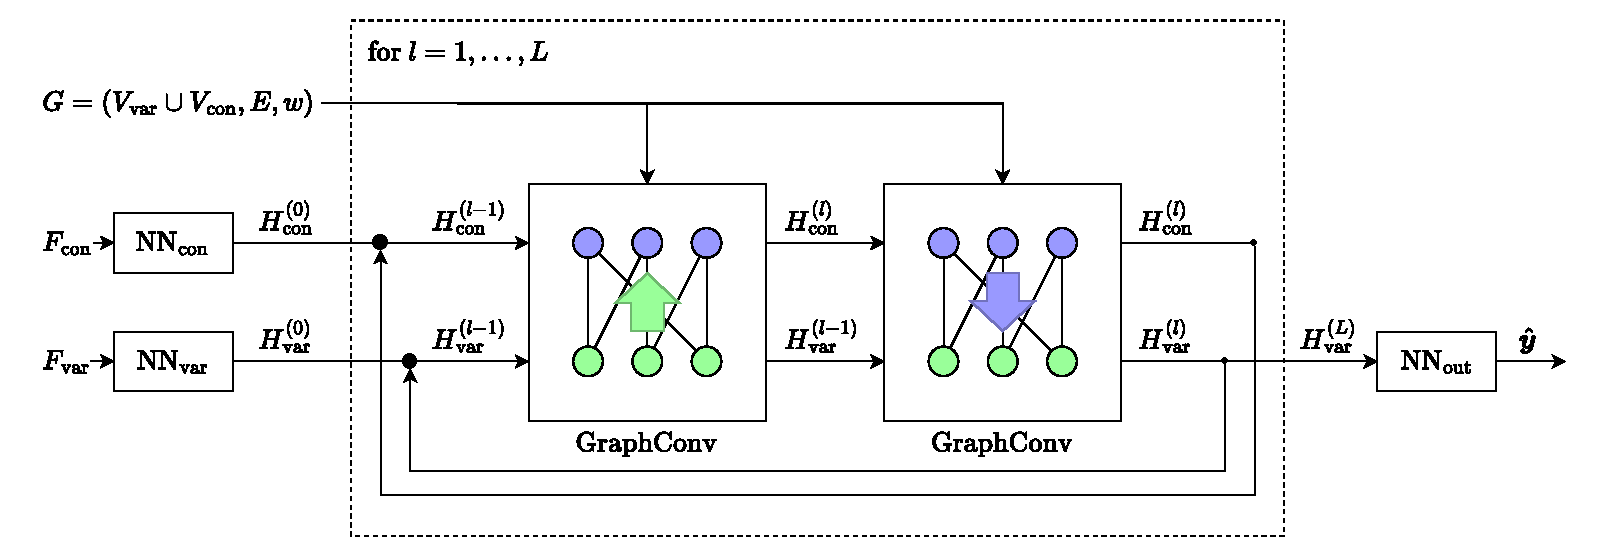
\includegraphics[width=\textwidth]{SatGNN.pdf}
    \caption{Architectural components of the solution prediction models trained for the ONTS problem. \emph{GraphConv} indicates the graph convolution operators as described in Sec.~\ref{sec:gnns}. $F$ and $H$ indicate sets of feature vectors. ${\rm NN}_{\star}$ are FCNs applied to each vector in the respective input set.}
    \label{fig:satgnn}
\end{figure}

Each layer of the proposed model performs the graph convolution in the form of two interleaved half-convolutions, as proposed by \citeonline{gasseExactCombinatorialOptimization2019} and widely adopted by similar applications~\cite{hanGNNGuidedPredictandSearchFramework2023,khalilMIPGNNDataDrivenFramework2022,dingAcceleratingPrimalSolution2020}.
The half-convolutions are applied to each partition of the graph, such that first the hidden feature vectors of the constraint nodes are updated using the hidden features of the variable nodes, and then the hidden features of the variable nodes are updated with the new hidden features of the constraint nodes.
These two operations are illustrated by the \emph{GraphConv} blocks in Fig.~\ref{fig:satgnn}.
The choice for the convolution operator is left as a hyperparameter, being either the FCN convolution proposed by \citeonline{kipfSemiSupervisedClassificationGraph2017} or the SAGE model proposed by \citeonline{hamiltonInductiveRepresentationLearning2017}, as discussed in Sec.~\ref{sec:gnns}.

After $L$ layers, the resulting hidden features are transformed into the predicted bias by another FCN.
The 2-layer network
\begin{align*}
    {\rm NN}_{\rm out}:\mathbb{R}^d_+& \longrightarrow \left( 0,1 \right)  \\
    \bm{h}^{(L)}_{v_{\rm var}} &\longmapsto \hat{p}_{v_{\rm var}} = {\rm NN}_{\rm out}(\bm{h}^{(L)}_{v_{\rm var}})
\end{align*}
combines each variable's output hidden features into a single value.
While the first layer has ReLU activation, the last layer has a sigmoid activation, constraining the output to the unit interval, which is adequate to the target range.

\section{Training}

The solution prediction models for the ONTS problem are trained with supervision to approximate the variable bias in the optimal solutions (see
Sec.~\ref{sec:training-solution-prediction}).
This approach is based on having a single (quasi-)optimal solution for each problem instance, and will be referred to in the following as \emph{OS} (Optimal Solution training).
Another approach is to exploit multiple near-optimal solutions, as discussed in Sec.~\ref{sec:multiple-targets}, training the model to approximate the variable bias of the solutions near optimal solutions.
This latter approach will be referred to as \emph{MS} (Multiple Solution training).
The dataset $\mathcal{D}$ built as described in Sec.~\ref{sec:data-acquisition} is used for both approaches, the only difference being that in OS the best solution is retrieved from $Z^{*}$, while in MS all solutions are used along with their objective value. 

As the ideal performance metric, i.e., the quality of the predicted solution, is not computable\footnote{In fact, it is not even defined over infeasible solutions.} for a vector of variable biases, the Binary Cross-Entropy (BCE) loss is used, as it is the loss of choice of the majority of works with similar applications~\cite{nairSolvingMixedInteger2021,hanGNNGuidedPredictandSearchFramework2023,khalilMIPGNNDataDrivenFramework2022,gasseExactCombinatorialOptimization2019}.
In MS, the BCE loss is weighed by a normalized value, which, as \citeonline{nairSolvingMixedInteger2021} has shown, is equivalent to the Kullback-Leibler divergence between the predicted variable biases and the actual variable biases of the near-optimal solutions.

For all experiments, Adam~\cite{kingmaAdamMethodStochastic2015} was used to perform stochastic gradient descent on the cost function (average BCE loss) over the training set.

\subsection{Hyperparameter Tuning}

Beyond usual hyperparameters from deep learning, such as learning rate and number of layers, the solution prediction model built for the ONTS problem has several hyperparameters that do not have well-established values in the literature.
Several experiments were performed to search for hyperparameter configurations that lead to the best solution prediction model for the ONTS problem.
The validation set was used for such experiments and the BCE loss was defined as the metric to be minimized.

The choice between the graph convolution operator proposed by \citeonline{kipfSemiSupervisedClassificationGraph2017} (henceforth referred to GCN) and the SAGE model is treated as a hyperparameter.
Early experiments with the SAGE model showed no benefits from complex aggregation functions such as an LSTM, as was proposed by \citeonline{hamiltonInductiveRepresentationLearning2017}.
In fact, from the aggregation functions proposed by the authors, the one that performed the best was the element-wise max-pooling.
The GCN graph convolution was implemented as proposed originally.

Considering the choice for graph convolution to apply to both half-convolutions (from variable nodes to constraint nodes, and from constraint nodes to variable nodes), it becomes possible to evaluate the effects of parameter sharing.
When parameter sharing is enabled, both half-convolutions are performed using the same parameters, instead of parameter vectors specific for that function.
Parameter sharing, also called weight tying, has been successfully applied to transformers (deep learning models based on the attention mechanism)~\cite{inan2017tying,press-wolf-2017-using}.
Due to the proximity between GNNs and transformers \cite{joshiTransformersAreGraph2020}, parameter sharing is evaluated in the context of the ONTS problem.

Beyond the choice for the graph convolution operator and whether or not to share the parameters, hyperparameters related to the model structure and the training are also taken into consideration.
Table~\ref{tab:hyperparameters} summarizes all hyperparameters considered for tuning along with value ranges, which were determined in early experiments on the validation set.
A random search was performed to select the best hyperparmeter configuration for OS and MS.
The configurations were used to train a model for 10 epochs on $\mathcal{D}_\textrm{train}$, after which the model was evaluated on the validation set.
Further implementation details and hyperparameter search results can be seen in this project's code repository\footnote{\url{https://github.com/gos-ufsc/sat-gnn}}.

\begin{table}[h]
    \centering
    \caption{Hyperparameters adjusted for the solution prediction models trained with either OS or MS for the ONTS problem. The columns  \emph{OS} and \emph{MS} present the best hyperparameter configuration found through random search for both training types.}
    \label{tab:hyperparameters}
    \begin{tabular}{l|c|c|c}
	\toprule
	Hyperparameter & Ranges & OS & MS \\
	\midrule
	Training & & & \\
	\quad Learning rate & $\left\{ 10^{-2}, 10^{-3}, 10^{-4} \right\} $   & $10^{-2}$ & $10^{-3}$ \\
	Architecture &  & & \\
	\quad Number of hidden features ($d$) & $\left\{ 2^{5},2^{6},2^{7},2^{8} \right\} $   & $2^{6}$ & $2^{8}$ \\
	\quad Number of layers ($L$)  & $\left\{ 1, 2, 3 \right\} $   & $2$ & $3$ \\
	\emph{GraphConv} &  & & \\
	\quad Operator & $\left\{ \text{GCN}, \text{SAGE} \right\} $   & SAGE & SAGE \\
	\quad Parameter sharing & $\left\{ \text{Yes}, \text{No} \right\} $   & Yes & Yes \\
	\bottomrule
    \end{tabular}
\end{table}

The hyperparameter configuration that resulted in the best model for both OS and MS is presented in Table~\ref{tab:hyperparameters}.
For both cases, the best model uses the SAGE function instead of GCN, although the best model found for MS is considerably bigger, with more layers and hidden features.
Note that both models also perform parameter sharing, suggesting that the proposed approach is effective.

\subsection{Final solution prediction models}

The best hyperparameter configuration found through random search for both OS and MS is used to train new models with a training budget of 100 epochs.
However, early-stopping is performed using the validation set, i.e., during the training, the model that performs the best on the validation set (over the epochs) is selected.
% Putting it into terms, the performance of the models on the validation set is evaluated during training.
% Then, the model with the lowest validation set cost is returned, which is effectively the same as stopping the training once the model achieves a minimum on the validation set over the epochs.
Early-stopping allows avoiding overfitting without the need to tune the training budget.
The training curves can be seen in Fig.~\ref{fig:opt-training-curves}.

\begin{figure}[h]
    \centering
    \begin{subfigure}{0.49\textwidth}
        \centering
        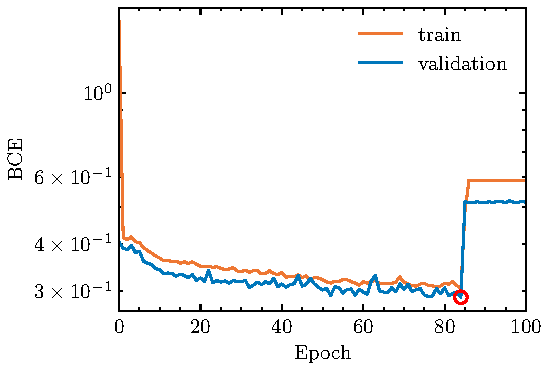
\includegraphics[width=\textwidth]{training_curve_optimal.pdf}
        \caption{Optimal Solution}\label{fig:training-bs}
    \end{subfigure}
    \begin{subfigure}{0.49\textwidth}
        \centering
        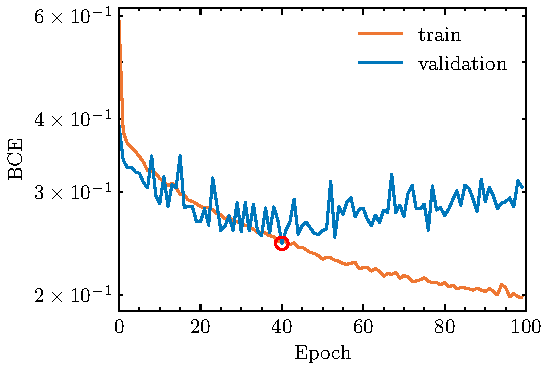
\includegraphics[width=\textwidth]{training_curve_multi.pdf}
        \caption{Multiple Solutions}\label{fig:training-ms}
    \end{subfigure}
    \caption{Training curves for the best solution prediction models trained through OS (a) or MS (b). The average BCE on the validation set is used for early-stopping the training (highlighted in red).}
    \label{fig:opt-training-curves}
\end{figure}

The model trained with OS achieved a validation cost of 0.2887 and a test cost of 0.2873, whereas the model trained with MS achieved a validation cost of 0.2451 and a test cost of 0.2482.
These values cannot be used to compare the training approaches, once the cost functions are different, but they indicate an absence of overfitting in both models, as the validation and test values are very close.
However, a comparison across training approaches can be performed when analyzing the confidence of the models on the test set.
A model's confidence is the predicted bias of the most likely assignment, i.e., in a binary problem, a model's confidence on the predicted value for the $j$-th variable is $\hat{p}_j$, if $\hat{y} = 1$, and $1-\hat{p}_j$ if $\hat{y}=0$.
To consider the entire test set, the confidence is measured at each time step, averaging over all tasks of all instances.
The result can be seen in Fig.~\ref{fig:prediction-confidences}.
It is possible to note that the MS model was, on average, much more confident of its predictions than the OS model.
Furthermore, both models provide significantly more confident predictions for the $\bm{\phi}$ variables than the $\bm{x}$ variables.

\begin{figure}[h]
    \centering
    \begin{subfigure}{0.49\textwidth}
        \centering
        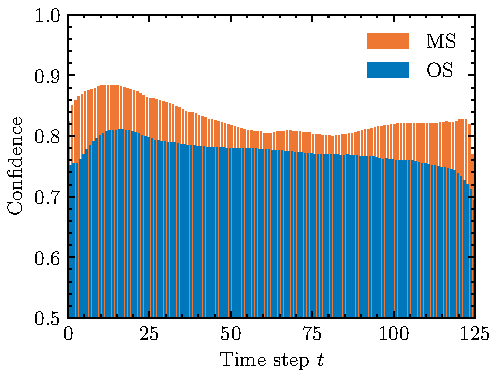
\includegraphics[width=\textwidth]{X_confidences.pdf}
        \caption{$x_{j,t}$}\label{fig:conf-x}
    \end{subfigure}
    \begin{subfigure}{0.49\textwidth}
        \centering
        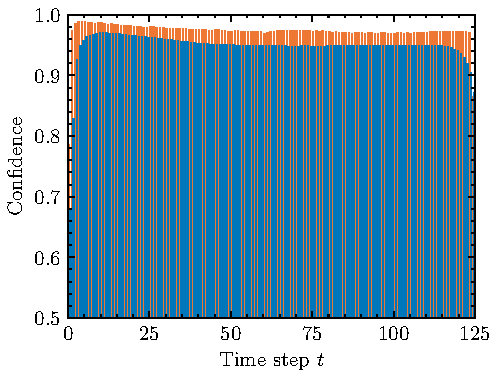
\includegraphics[width=\textwidth]{Phi_confidences.pdf}
        \caption{$\phi_{j,t}$}\label{fig:conf-phi}
    \end{subfigure}
    \caption{Average confidence of predicted values for (a) $\bm{x}$ and (b) $\bm{\phi}$ variables of the models trained via OS and MS. Each bar is the average confidence over the predictions for all tasks $j$ of all instances $I$ in the test set.}
    \label{fig:prediction-confidences}
\end{figure}

\section{Learning-based heuristics}

The two solution prediction models (the one with OS and the one with MS) were each used to build three primal matheuristics.
Namely, warm-starting, early-fixing and trust-region, as per Sec.~\ref{sec:learning-based-heuristics}.
As these matheuristics have hyperparameters of their own, another set of experiments was performed to find the best values for these hyperparameters.
The matheuristics were evaluated considering two possible goals: reducing the time to find a feasible solution, and finding the best solution under 2 minutes.
Both goals are directly related to finding a new schedule during the communication window of the nanosatellite's orbit, as detailed in Sec.~\ref{sec:instance-space}.
Therefore, each model is tuned and evaluated with respect to both goals.
The SCIP solver is used both as the baseline and within the matheuristics.

\subsection{Tuning}

All three matheuristics implemented are based on partial solutions, thus, naturally, the size of the partial solution can be seen as a hyperparameter, which can be adjusted through the confidence threshold.
On top of that, the trust-region method also has the radius $\Delta\in \mathbb{N}$.

Two sets of experiments are performed for each model using the validation set.
For once, the hyperparameters are adjusted with the goal of reducing the average time to find a feasible solution.
In parallel, the hyperparameters are adjusted to maximize the average relative objective value (QoS) during a 2-minute time budget.
For each instance, the resulting objective values are normalized by the known maximum, following Equation~\eqref{eq:relobj}, but assuming that the trivial solution has 0 objective.
This ensures all instances have equal influence in the aggregated value.
Because there are few hyperparameters to be tuned, the experiments were performed manually, ensuring equal effort was dedicated to all models and resulting heuristics.
The best values found are reported in Table~\ref{tab:best-N-delta}.

\begin{table}[h]
    \centering
    \caption{%
	Best values for partial solution size $N$ and trust-region radius $\Delta$ (when applicable) for each heuristic resulting from both solution prediction models (either trained via OS or MS).
	Columns \emph{Objective} indicates the values that maximized the relative objective value in the validation set, while columns \emph{Feasibility} indicate the values tuned to minimize the time taken to find a feasible solution.
 }
    \label{tab:best-N-delta}
    \begin{tabular}{ll|cc|cc}
    \toprule
    \multirow{2}{2cm}{Training Approach} & & \multicolumn{2}{c|}{Objective} & \multicolumn{2}{c}{Feasibility} \\
                            & Heuristic    & $N$         & $\Delta$        & $N$          & $\Delta$         \\
    \midrule
    \multirow{3}{*}{OS}      & Warm-start   & 750         & -               & 1000         & -                \\
                                        & Early-fix    & 500         & -               & 750          & -                \\
                                        & Trust region & 1000        & 5               & 1000         & 1                \\
    \midrule
    \multirow{3}{*}{MS} & Warm-start   & 1750        & -               & 1500         & -                \\
                                        & Early-fix    & 1000        & -               & 1250         & -                \\
                                        & Trust region & 1250        & 1               & 1750         & 1             \\
    \bottomrule 
    \end{tabular}
\end{table}

\subsection{Evaluation}

The heuristics with the best partial solution size and trust-region radius (Table~\ref{tab:best-N-delta}) are evaluated on the test set, which was not used in any tuning experiment.
The models are evaluated with respect to both goals, following the same metrics as for the heuristic hyperparameter tuning experiments, namely, the average time to find a feasible solution and the average relative objective value, under a 2-minute budget.
Note that the objective values are normalized following Equation~\eqref{eq:relobj}, with the optimal solution being the best known solution of each instance, but with an "artificial" trivial solution that has null objective (i.e., $QoS=0$ ).
A null objective is also assumed if the instance is deemed infeasible or as long as the solver cannot find a feasible solution.
The progress of the relative lower bound (relative objective of the candidate solution over time) is also measured within the time budget to evaluate how the heuristics perform for smaller budgets.
The performance of each heuristic in the test set is presented in Figure~\ref{fig:heuristics-test-results}.

\begin{figure}[h]
    \centering
    \begin{subfigure}{0.99\textwidth}
        \centering
        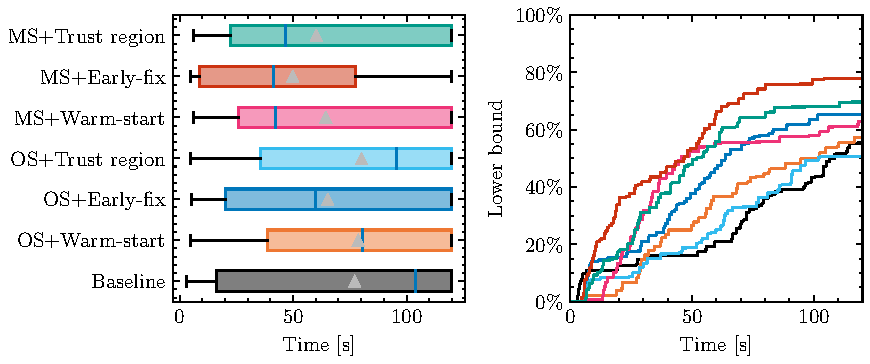
\includegraphics[width=\textwidth]{heuristic_test_feas.pdf}
        \caption{Time to find a feasible solution (lower is better).}
        \label{fig:heuristics-test-results-feas}
    \end{subfigure}
    \begin{subfigure}{0.99\textwidth}
        \centering
        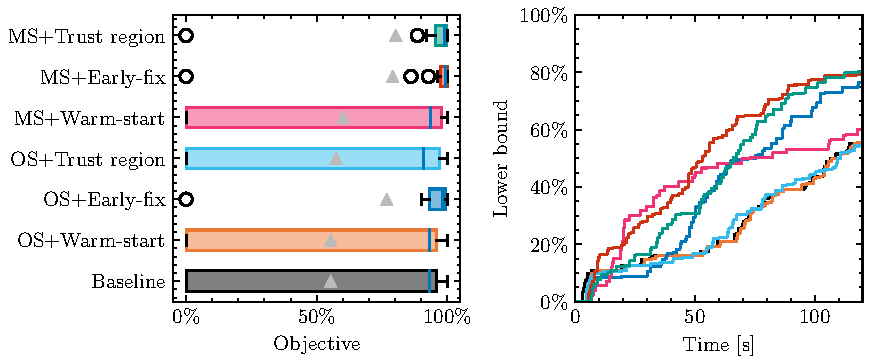
\includegraphics[width=\textwidth]{heuristic_test_obj.pdf}
        \caption{Normalized objective value within 2 minutes (higher is better).}
        \label{fig:heuristics-test-results-obj}
    \end{subfigure}
    \caption{%
    Test performance of the learning-based heuristics for the ONTS problem.
    In (a), the boxplots show the quartiles and outliers (circles) of the values that correspond to the heuristics adjusted to minimize the average time to find a feasible solution (on the validation set).
    The vertical blue lines indicate the medians, while the triangle icons indicate the average values.
    In (b), the heuristics used were those adjusted to maximize the average relative objective value (also on the validation set).
    The box plots show the distribution of the metric of interest (time to find a feasible solution in (a), and relative objective value in (b)) over the test set, with the small triangle indicating the average value.
    The plots on the right show the progress of the relative lower bound (relative objective value of the candidate solution) during the 2 minutes time budget, averaged over all instances of the test set.
    % On the left, we have the distribution of the evaluation metric of interest over the instances of the test set for the multiple approaches, in which the triangle indicates the mean value and the circles indicate outliers. \emph{MS} indicates that the SatGNN model trained with multiple solutions was used, whereas \emph{OS} indicates that the model trained solely with the optimal solution was used instead. On the right is the average progress of the lower bound on all test set instances. The objective value is considered relative to the known optimal value; thus it always lies in the unit interval. The heuristics' hyperparameters $N$ and $\Delta$ are defined upon experiments on the validation set, as presented in Table \ref{tab:best-N-delta}.
}
    \label{fig:heuristics-test-results}
\end{figure}

The results indicate that most of the learning-based heuristics provide a clear improvement over the baseline approach of using the SCIP solver, given the limited time budget.
To assess the statistical significance of the gains, the Wilcoxon signed-rank test~\cite{wilcoxon_1945} was applied to the test set results.
The Wilcoxon signed-rank test is a non-parametric version of the Student's t-test for matched pairs, which implies that normality is not assumed for the distribution of the metrics\footnote{This is particularly important for the relative objective value, which is highly skewed and limited to unit interval.}.
The test is applied in pairs, comparing each matheuristic to every other, including the baseline.
The results of the statistical significance test are summarized in Figure~\ref{fig:cdds}.

\begin{figure}[h]
    \centering
    \begin{subfigure}{0.99\textwidth}
        \centering
        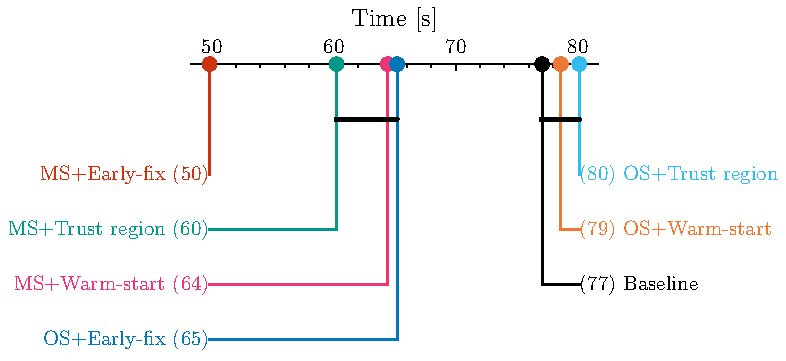
\includegraphics{cdd_feas.pdf}
        \caption{Time to find a feasible solution (lower is better).}
        \label{fig:cdd-feas}
    \end{subfigure}
    \begin{subfigure}{0.99\textwidth}
        \centering
        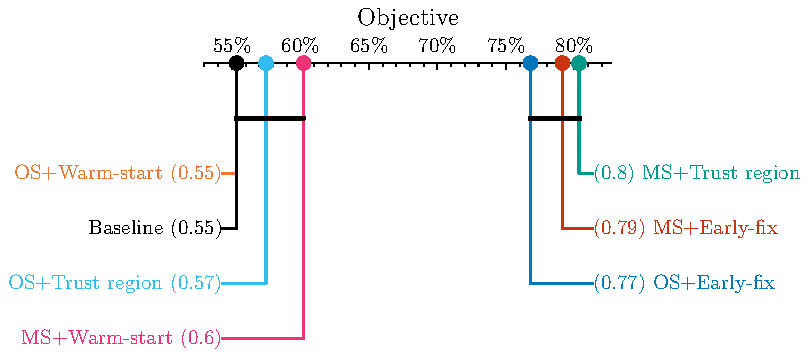
\includegraphics{cdd_obj.pdf}
        \caption{Normalized objective value within 2 minutes (higher is better).}
        \label{fig:cdd-obj}
    \end{subfigure}
    \caption{%
    Critical difference diagram of the test set performance of the learning-based heuristics for the ONTS problem.
    Figures (a) and (b) show the performance of heuristics adjusted for minimizing the time to find a feasible solution and maximizing the relative objective value within a 2 minute budget, respectively.
    The round marker in the axes indicates the heuristic's average performance.
    A crossbar connecting multiple approaches indicates that their performance (distribution on the test set) was not significantly different ($p$-value $>0.05$) in the paired Wilcoxon signed-rank test.
%presenting the average test set performance of the SatGNN-based matheuristics (round marker in the axis). A crossbar between two (or more) approaches indicates that their performance (distribution on the test set) was not deemed significantly different ($p$-value$>0.05$) through the paired Wilcoxon signed-rank test~\citep{wilcoxon_1945}.
    }
    \label{fig:cdds}
\end{figure}

For both goals, the early-fixing matheuristics were able to significantly overcome the baseline.
In particular, using the solution prediction model with MS to perform early-fixing provided the most consistent results, being not only significantly better than the baseline, but also significantly better than all other heuristics on the goal of finding a feasible solution the fastest.

